%!TEX root = /Users/markelikalderon/Documents/Git/timaeus/timaeus.tex
\chapter{The End of Vision and Audition} % (fold)
\label{cha:the_end_of_vision_and_audition}

\section{A Sensory Soteriology} % (fold)
\label{sec:a_sensory_soteriology}
The Circles of the Same and the Different in the immortal part of the human soul are waverable. The shock of embodiment of a newly incarnate soul disrupts their motions, as well as the kinaesthetic and cognitive powers that these motions determine. The experience is disorienting and traumatic. Fortunately, the disruption incurred by the shock of embodiment is providentially accommodated. The young gods, acting on behest of the Demiurge, provide human beings with the sensory powers of vision and audition. In exercising these powers on the right objects, in the right way, and in concert with other powers, the Circles of the Same and the Different may return, over time, to their proper revolutions. In observing the revolution of the Heavens, we see the motion of a visible god, a visible manifestation of divine thought. The fixed stars revolve around the Circle of the Same whereas the wanderers, the planets, revolve around the Circle of the Different. In aligning the waverable motions of the Circles of the Same and the Different in the human soul with the unwaverable motions of the Circles of the Same and the Different in the World-Soul, reason and virtue are restored. 

There is a limited egalitarianism in Timaeus' soteriology. Any human being equip\-ped with the sensory powers of vision and audition is providentially provided for. In this way is the soteriology egalitarian. Timaeus' soteriology, however, is limited in two ways. It is limited, first, in not being automatic and, second, in not being available to every sentient being. First, it is not automatic. Being equipped with these sensory powers is not sufficient for salvation. They must be exercised on the right objects, in the right way, and in concert with other powers, over an extended period of time. Second, not every sentient being has the auxiliary powers that must be exercised in concert with vision and addition. Non-rational living beings, such as non-human animals, lack the relevant auxiliary powers. Sheep do not calculate the motion of the stars. The young gods, on behest of the Demiurge, provide specifically humans with the opportunity for salvation. Taking them up on that opportunity nonetheless requires a sustained and concerted effort.

% section a_sensory_soteriology (end)

\section{Vision} % (fold)
\label{sec:vision}
Timaeus' discussion of vision is structured as follows:
\begin{enumerate}[(1)]
	\item The young god's creation of the body proper to the day and the eye from the same kind of fire (45a6--45c3; subsection~\ref{sec:the_eye_and_the_body_proper_to_the_day})
	\item The compounding of the visual body when the fire emanating from the eye meets what is like it, the body proper to the day (45c3--45d3; subsection~\ref{sec:the_compounding_of_the_visual_body})
	\item The extinguishing of the fire emanating from the eye when it meets what is unlike it, the dark air of night (45d3--45d7; subsection~\ref{sec:the_quenching_of_the_eye_s_fire})
	\item An explanation of sleep and dreams (45d7--46a2; subsection~\ref{sec:sleep_and_dreams})
	\item A catoptrics (46a3--46c6; subsection~\ref{sec:timaen_catoptrics})
	\item A methodological digression on causes, \emph{aitia}, and auxiliary causes, \emph{sunaitia} (46c7--46e6; subsection~\ref{sec:_emph_aitia_and_emph_sunaitia})
	\item Observing the revolutions of the Heavens and the end of sight (46e7--47c4; subsection~\ref{sec:the_end_of_sight})
\end{enumerate}
Though complex, this is merely a preliminary discussion of vision. Timaeus will take up the proper object of vision, color, later on in his speech (67c–68d) when discussing the affections (\emph{pathēmata}) peculiar to particular parts of the body (65b–68e). There, he will also give some additional detail about the anatomy of the eye, more fully specify the affections that colors produce in the eyes, as well as provide an account of color mixture that rivals Democritus'. Moreover other aspects of Timaeus' discussion of the \emph{pathēmata} are relevant to his general conception of perception and so are applicable to vision. Particularly, with respect to the \emph{pathēmata} common to the body as a whole (61d–65b, chapter~\ref{cha:common_pathemata}), his discussion of pleasure and pain (64a2–65b3, chapter~\ref{sec:pleasure_and_pain}) makes a general claim about the nature of the recipient of the relevant affection and so is applicable to vision. Moreover, it is only within the context of Timaeus' discussion of the \emph{pathēmata} as a whole, both common and peculiar, does Timaeus' conception of perception as a kind of measure clearly emerge. On that conception, a \emph{pathēma} is the measure of the power of the agent that produced it, and perception is a cognizance of this power. Our understanding of Timaeus' account of vision is incomplete unless it is set against this larger background.

 % And with respect to the \emph{pathēmata} peculiar to particular parts of the body (65b–68e, chapter~\ref{cha:peculiar_pathemata}), his discussion of the ears (67a–c, chapter~\ref{sec:the_ears}) makes general claims about perception (as \citealt{Barker:2000dy} and \citealt{Lautner:2005aa} argue) and so are applicable to vision.

% section vision (end)

\section{The Eye and the Body Proper to the Day} % (fold)
\label{sec:the_eye_and_the_body_proper_to_the_day}

The young gods present task is the construction of the face, the forward part of the vessel of the head. The face is arrayed with organs for the forethought of the soul, and the eyes are the first of the organs that the young gods construct. How are the eyes organs for the forethought of the soul? And why are they a priority for the young gods? Forethought, here, carries suggestions of distance and time. If one can see something in the distance one can reason how best to act in the time before encountering it (Calcidius, \emph{In Timaeum} 230.). This may be of vital concern should what is seen be predator or prey. Thus Alcinous speaks of the senses as guardians of the ruling part (\emph{Didaskalikos} 17 173.10). Though strictly non-Platonic, the aptness of the image is manifest in the frequency with which it is repeated (see, for example, Philo, \emph{De opificio mundi} 139, \emph{Legum Allegoriarum} 3 115, Galen, \emph{De placitis Hippocratis et Plotonis} 2.4 120, and Calcidius, \emph{In Timaeum} 231.) Timaeus is hinting right at the beginning that vision is a great benefit to humanity. Moreover, as we shall see, the benefit is not narrowly confined to its survival value. The temporal implications of forethought are especially important. By means of vision we have a view of the revolutions of the Heavens and so can distinguish days and nights, months, and years. In observing these we acquire number and even greater feats of forethought are made possible both in agriculture and seafaring. In exercising our reason in acquiring and deploying number we become capable of engaging even in philosophy. Moreover, in so doing we align the Circles of the Same and the Different in the immortal part of our soul with the Circles the Same and the Different in the World-Soul whose movement is visibly manifest in the revolution of the Heavens. We see divine thought visibly manifest and thus may offset the disturbing effects of the shock of embodiment. In this way is vision the greatest benefit that the gods bestow upon us. Notice that in answering our first question, concerning the eyes as organs for the forethought of the soul, we have also answered our second question, concerning the priority of the eyes. The eyes are a priority for the young gods precisely because they are the greatest benefit to humanity. This issue of priority will be echoed in Timaeus' later discussion of the affections peculiar to particular parts of the body (65b–68e), for there, he will discuss the parts of the body whose affection is liable to give rise to perception or sensation in ascending order of ethical significance culminating with the eyes (chapter~\ref{sec:common_versus_peculiar_pathemata}).

The Timaean anatomy of the eye is broadly Empedoclean (DK 31B84--88). Each represents the eye as the product of divine craftsmanship, with the young gods in Timaeus' account playing Aphrodite's role in Empedocles'. Each maintains that there is a fire in the eye, likened to light, that flows through the center owing to its fineness. Thus the organs that the young gods affix to the face are said to be light-bearing eyes (\emph{phōsphora ommata}). Though Empedocles does not use the adjective, \emph{phōsphora}, the lantern analogy (Aristotle, \emph{De sensu} 2 437b27–438a3 = DK 31B84) clearly implies that eyes are, in fact, light-bearing (in some sense or another, depending upon how that analogy is to be understood). A variant form of that adjective, \emph{phaesphorōi}, is also applied to the eye in Euripides' \emph{Cyclops} 462 (see \citealt[489-90]{Seaford:1984vb} and \citealt[114]{Johansen:2004dx}). In a cruel irony, Odysseus, in describing his plan to blind the Cyclops with a fiery brand, says that the Cyclops' eye shall be truly light-bearing. Notice that the irony only gets a grip against the background of some view, like Empedocles', that the eyes anyway bear light, though perhaps not in the way that the Cyclops' will. This is a view that Timaeus shares not only with Empedocles, but also Alcmaeon of Croton (see \citealt[11--13]{Beare:1906uq}), and it was widely enough held to be the basis for Euripides' irony in his satyr play.

In his discussion of the \emph{gēne}, Timaeus claims that there are many kinds of fire and gives three examples though he does not claim that these exhaust the kinds of fire that there are (58c5–d1). First, there is flame (\emph{phlox}). Second, there is the kind that issues from flame but does not burn but supplies light to the eyes (in Latin, \emph{lux} as opposed to \emph{lumen}). And third, there is the kind that is left behind in embers after the flame is extinguished. The young gods contrive daylight, a body proper to each day, out of the second kind of fire, that gives a mild light but does not burn (45b4--6). There is a play on words here that hints at an etymology. The Greek word for day, \emph{hemeras}, clearly echoes the adjective, \emph{hemeron}, that means mild. In the \emph{Cratylus} (418c--d), Socrates spurns the etymology that takes \emph{hemeron} as the root of \emph{hemeras} preferring the older etymology that takes \emph{himera} as the root. So understood, it is not the mildness of its light by which the day is called but our longing for this light after the dark of night. Both resonances may be in play here. Timaeus may be emphasizing both the mildness of the day's light and our longing for it. Timaeus will argue that the mild light proper to the day is necessary for vision. It is among the auxiliary causes (\emph{sunaitia}) of vision. But the longing for light naturally motivates our looking toward the celestial clockwork and so contributes to the end of sight as well. And just as Socrates suggests that the older etymology provides us with a deeper understanding of the significance of \emph{hemeras}, the longing for light, given its connection with providential end of sight, promises to provide us with a deeper understanding of vision. Indeed, this is an instance of a methodological point that Timaeus himself makes, looking to the \emph{aitia} one gains a better understanding of the \emph{sunaitia}.

Daylight, then, is a body proper to the day composed of a mild light that does not burn. The fire within the eye is said to be akin, \emph{adelphon}, literally brother, to the mild light of the day (so like the English ``akin'', \emph{adelphon} may convey either similarity or familial relationship). Being sons of the same mother, the fire within the eye and the daylight without belong to the same family. Perhaps Timaeus is suggesting in this way that each is the same kind of fire, that gives a mild light but does not burn. I hedge only because Timaeus stops just short of making this claim explicit. It is nonetheless plausible that the fire within the eye is mild and does not burn since, if it did, the eye would be damaged, as the fire of Odysseus' brand damages the Cyclops' eye. Timaeus himself will give an example of this kind. Brilliant (\emph{stilbon}) bodies emit a flame whose particles enter the passages in the eye and dissolves them and the dazzling experience they give rise to blinds the perceiver to details of the scene before them (chapter~\ref{sec:the_eyes}). Beyond its kinship with daylight, it is independently plausible, then, in the framework of the Timaeus, that the fire within the eye is of the kind that does not burn.

\citet[112]{Johansen:2004dx} makes a complementary suggestion. Light-bearing eyes and the Sun not only emit a mild light that does not burn, but they share a common \emph{aitia}, the young gods generate each for the sake of the same good (discussed further in section~\ref{sec:_emph_aitia_and_emph_sunaitia}). The fire emanating from within the eye and the body proper to the day are thus alike not only in being a mild light that does not burn, but they are also alike in that their sources are providentially provided for a common purpose. As we shall see in the next section, both dimensions of similarity are relevant, in different ways, to the compounding of the visual body (\emph{opsis}) from the fire emanating from within and the body proper to the day.

The \emph{Chaldean Oracles} are thus wrong, if understood as a Middle Platonist interpretation of the \emph{Timaeus} (see \citealt{Brisson:2003aa}):
\begin{quote}
	Do not measure the extent of the sun by joining rods together, for he is borne along by the eternal will of the Father and not for your sake. (\emph{Chaldean Oracles}, Fragment 107; \citealt[89--91]{Majercik:2013jw})
\end{quote} 
The \emph{Chaldean Oracles} are meant to be a record of Plato's doctrines revealed by Plato himself to Julian the Theurgist as a result of theurgic activity, sometime during the reign of Marcus Aurelius. The present discrepancy should not deter us, however. Julian seems to reject Timaeus' sensory soteriology in favor of a soteriology based on theurgic activity involving the uses of corporeal symbols in rites to invoke divine powers (see \citealt[21--25]{Majercik:2013jw} for discussion). The discrepancy is motivated by the religious inovation of the intervening centuries.

The young gods cause this fire within, brother to daylight, to flow through the eyes (45b6--c2, for the grammar of this passage see \citealt[63 123--127]{Cook-Wilson:1889cs} and \citealt[277]{Taylor:1928qb}). With this in mind, they compacted the whole of the eye and made its center, presumably the pupil or perhaps the cornea, especially smooth and dense so as to only allow the internal fire to escape, owing to its fineness, while keeping within all that is coarser. (Following \citealt[125--6]{Cook-Wilson:1889cs}, \citealt[277]{Taylor:1928qb} and \citealt[152]{Cornford:1935fk}, I take \emph{leion kai puknon}, smooth and dense, to modify \emph{holon} and \emph{to meson} rather than \emph{rhein} so that the stream of fire flows through a smooth and dense eye or its center rather than the stream itself being smooth and dense. Alcinous, \emph{Didaskalikos} 18 20, makes this mistake, but Calcidius gets it right in his Latin translation, \emph{In Timaeum} 46c.) This closely corresponds in description and function to the screen of shaved horn, or perhaps of flaxen linen (see \citealt[240--1]{Wright:1981zr}), in Empedocles' lantern analogy (Aristotle, \emph{De sensu} 2 437b27–438a3 = DK 31B84). The center of the eye is an efficient filter. Only the finest and purest of fire is said to escape. The fire emanating from within is said to have two consequences depending upon the occasion. When it is day, the fire emanating from within meets what is like it and forms a compound with the daylight, and when it is night and the body proper to the day withdraws, it meets what is unlike and is quenched and so extends no further. Let us consider these in turn.

% section the_eye_and_the_body_proper_to_the_day (end)

\section{The Compounding of the Visual Body} % (fold)
\label{sec:the_compounding_of_the_visual_body}

When it is day, the fire within goes forth like to like (\emph{homoion pros homoion}). The fire within is brother to the daylight and is like it in being a mild light that does not burn. So when it is day, the fire emanating from within meets what is like it. This is why the young gods contrived the body proper to the day as they did. This encounter of like with like has an important consequence. The fire emanating from within is compacted with the daylight (\emph{sumpages}, appearing in the text as {\sbl ξυμπαγές} as opposed to {\sbl συμπαγές}). This happens in whatever direction the perceiver is looking when the internal fire comes into contact with an external body. In compacting the two fires thus form a unified homogenous body (\emph{hen sōma oikeiōthen}) and so the sons of the same mother come to share a common household. And as this is the purpose of the young gods in contriving both to be like, it is a providential union. Later, not only are the two fires said to be compacted but also grown together (\emph{sumphues} appearing as {\sbl ξυμφυὲς}, 64d8), further emphasizing that the compound is a unified body. And as each fire is a mild light that does not burn, presumably, so too is their compound. This unified homogenous body is aligned in the direction in which the eyes are looking. So Timaeus reifies lines of sight, conceiving of them as a unified homogenous bodies compounded from the fire within and the daylight that it encounters in the direction that the perceiver is looking (see Plutarch's paraphrase in \emph{Quaestiones convivales} 1.8.4). In Greek, ``\emph{opsis}'' means vision or sight and yet Timaeus will use this term to refer to the body compounded of internal and external fire. Following \citet[221]{Ierodiakonou:2005ly}, I shall refer to the compound as the visual body.

The principle governing the compounding of the visual body is like's affinity for like. We should not confuse this with another application of this principle in the vicinity. It is the compounding of the visual body, an auxiliary cause of vision, and not vision itself that is governed by the principle of like's affinity for like. In \emph{De anima} (1.2 404b7--15), Aristotle claims that Empedocles explains perception by like's affinity for like, citing the following passage as evidence:
\begin{verse}
	By earth we see earth; by water, water;\\
	by aither, shining aither; but by fire, blazing fire;\\
	love by love and strife by baneful strife (Empedocles DK 31B109; \citealt[221]{Inwood:2001ve})
\end{verse} 
(This is controversial, however, see \citealt{Kamtekar:2009fk}.) Aristotle goes on to claim that Timaeus, like Empedocles, similarly explains perception in terms of the principle of like's affinity for like (\emph{De anima} 1.2 404b16--9). But, in the present passage at least, Timaeus has in mind a more limited application of this principle. The principle is only invoked to explain the compounding of the visual body. Sight only occurs when the visual body is affected as a whole and this affection is conveyed to the body where it reaches the soul. So there are further phases in the causal process eventuating in perception subsequent to the compounding of the visual body. Thus it is only the compounding of the visual body, a necessary if insufficient condition for perception, and not the perception that may eventuate, that is here being explained. Not only is the application of the principle, like's affinity for like, limited in this way, but there is a further difference between Timaeus and Empedocles as well. Light plays no role in Empedocles' account of vision, but plays an indispensable role in Timaeus' account. Aristotle, of course, will follow Timaeus in this (\emph{De anima} 2.7 418b3).

That the fire emanating from within the eye and the body proper to the day are alike in being a mild light that does not burn is what makes the principle of like's affinity for like operative in compounding the visual body. \citet[112]{Johansen:2004dx} made a complementary suggestion (discussed in section~\ref{sec:the_eye_and_the_body_proper_to_the_day}). They are also alike in that the young gods generate their sources, the eye and the Sun, for the sake of the same good. If that is right, then the fact that the two fires are of the same kind, thus allowing the principle of like's affinity for like to compound them into the visual body, is the work of divine providence.

Light may be an indispensable condition for vision, but Aristotle and Timaeus disagree about why this may be so. For Timaeus, the body proper to the day is an indispensable condition for vision since it is a part of the compound through which the motion from the visible object is communicated to the body before it reaches the soul. Aristotle, however, finds the compounding of the visual body puzzling (\emph{De sensu} 2 438a29ff). He begins by distinguishing two views both of which are unreasonable (\emph{alogon}). On the first view, the emission from the eye reaches as far as the body seen, even as far as the stars. Alexander of Aphrodisias attributes this view to the ``mathematicians'' (\emph{In librum De sensu commentarium} 27.28--28.7), presumably the tradition of geometrical optics that included Archytas of Tarentum (if Apuleius is to believed, \emph{Pro se de magia} 15, see \citealt{Burnyeat:2005rc}), Hero, Euclid, and Ptolemy. Thus, for example, in the first definition of his \emph{Optics}, Euclid claims that lines from the eye extend a great distance, and in his third definition, he claims that those things upon which they fall are seen. On the second view, the emission from the eye extends only a certain distance and grows together (\emph{sumphues}) with the light. Aristotle's attribution of this second view is non-specific, ``as some say'', but he clearly has Timaeus in mind (see also Theophrastus' paraphrase, \emph{De sensibus} 5). The locution's generality suggests that Aristotle's target is all those, within the Academy and without, who share Timaeus' view.

With respect to the first view, if the emission is corporeal, Aristotle doubts whether the eye contains enough substance to extend great distances, even as far as the stars. Later, Malebranche will echo Aristotle's worry when he writes:
\begin{quote}
	We see the sun, the stars, and an infinity of objects external to us; and it is not likely that the soul should leave the body to stroll about the heavens, as it were, in order to behold all these objects. (Malebranche, \emph{Recherche de la V\'{e}rit\'{e}}, 3.2.1.1; Thomas M. Lennon and Paul J. Olscamp, \citeyear[217]{Malebranche:1997sf})
\end{quote}
Whereas Malebranche is worried about the locomotion of the soul, Aristotle is worried, not about locomotion, but about growth. Aristotle doubts that the body of the eye contains enough for an interior component of it to grow so as to extend even as far as the stars. Even if the eye's corporeal emission were sufficiently rarefied to extend great distances, they would be easily disturbed, by a wind say. But our sight is not disturbed in this way.  (For these and other difficulties see Alexander of Aphrodisias, \emph{In librum De sensu commentarium} 27.20--30.29, Aquinas, \emph{Sentenciae libri De sensu et sensato} 3.) Unlike the mathematicians, however, Timaeus does not claim that the fire emanating from within extends to the body seen. And so his account is not subject to these, and related, difficulties.

With respect to the second view, Aristotle says that it would be better if the coalescence occurred at the surface of the eye rather than at a certain distance (\emph{De sensu} 2 438a28--9). Why would it be better? There are two cases to consider. Either daylight extends to the surface of the eye or it does not. In the latter case, the fire emanating from within would meet darkness and would be extinguished, at least by Timaeus' lights (Alexander of Aphrodisias, \emph{In librum De sensu commentarium} 32.23--24, Aquinas, \emph{Sentenciae libri De sensu et sensato} 3). And if the light extends to the surface of the eye, then it would be unnecessary for it to travel further, even a certain if not a great distance (Aquinas, \emph{Sentenciae libri De sensu et sensato} 3). This last point may be questioned, however. Perhaps in order to compact and grow together, the fire emanating from within must extend a certain distance into the daylight.

At this point, Aristotle raises general and specific puzzles about the compounding. The general puzzle is expressed by his query how can light coalesce with light? While Timaeus conceives of light as aggregates of fire particles and so as corporeal, Aristotle denies that light is a body (\emph{De anima} 2.7 418b21--7), claiming instead that it is a state (\emph{hexis}). Perhaps, Aristotle's thought, here, is that while bodies may be mixed or separated, states cannot be (\emph{De generatione et corruptione} 1.10 327b20--1, Alexander of Aphrodisias, \emph{In librum De sensu commentarium} 33.9--12, Aquinas, \emph{Sentenciae libri De sensu et sensato} 3). \citet[140--1]{Ross:1906xi} criticizes the Alexandrian interpretation since ``\emph{sumphues}'' means grow together or coalesce and not mixing. Two observations are relevant here. First, it is not unreasonable that a Peripatetic would reconstrue the Platonic thought in this way. Second, a Peripatetic might reply to Ross that, just as states do not mix, neither do they grow together. Aristotle's worry, here, however it may be understood, depends upon his conviction, that Timaeus rejects, that light is incorporeal. Aquinas offers an additional reason for Aristotle being puzzled about light coalescing with light (\emph{Sentenciae libri De sensu et sensato} 3). It would not be possible for the internal and external fire to be compacted and grown together to form a unified homogenous body since they are not of the same nature. This latter claim is what Aquinas takes Aristotle to mean by saying that not just any body may coalesce (\emph{De sensu} 2 438b). Not just any body may coalesce, only those that share a common nature may do so. But Timaeus does, in fact, claim that they are of the same nature, and so absent a reason for doubting this, Aristotle's puzzlement, on the Thomistic reading, is no puzzlement at all. 

Assuming that the compounding of the internal and external fire is best understood to happen at the surface of the eye, Aristotle raises a further more specific puzzle, for surely they are separated by a membrane that corresponds to the screen in Empedocles' lantern analogy (Aristotle, \emph{De sensu} 2 437b27–438a3 = DK 31B84). This is distinct from the general puzzle. Even should it be intelligible that light may coalesce with light, the membrane separating internal and external light would surely prevent this. Empedocles and Timaeus would reject such an objection as unfounded since they postulate passages in the eye through which only the finest and purest fire may flow. And it is through such passages that internal and external light may grow together. Overall, it would seem, then, that the Aristotelian objections work better on their own terms than on Timaeus'.

Since internal and external fire are compacted and grown together to form a unified homogenous body, this body, the visual body, is affected as a whole. Moreover it is the principle of its compounding, like's affinity for like, that explains this. It is because the visual body is uniformly formed that it is uniformly affected (\emph{homoiopathes dē di homoiotēta}). (The unity and homogeneity of the visual body and its consequences for how it may be affected is usefully compared to the role of sympathy in uniting \emph{eidola} emanating from sensible objects in Epicurus' \emph{Letter to Herodotus}, see \citealt{Lee:1978yz}.) In his discussion of pleasure (64a2--c7), Timaeus explains that the communication of the affection depends upon the mobility of the particles which compose the relevant part of the body. Fire particles are particularly mobile, and so it might be thought that the affection is communicated through the visual body owing to the mobility of its constituents. But the present discussion of vision suggests an alternative model. The visual body is a unified homogenous body that is uniformly affected. It is this unified body as a whole that receives the affection which it passes on to the body before reaching the soul (45c--d; see \citealt[72, 92 n46]{Hahm:1978ny} for discussion). So the affection is not communicated part by part within the visual body as one might be tempted to think. The mobile nature of the recipient would seem only to apply to the way the visual body as a whole passes around the affection to the rest of the body before it reaches the soul.

This bears on the proper interpretation of the visual body (\emph{opsis}). Timaeus understands the sensitivity of a member in terms of the mobility of the parts that compose it, and the fire particles that compose the visual body are especially mobile. If on this basis, one understood the affection or motion as being communicated part by part though the visual body, then the visual body, so conceived, would be sensitive throughout. By this means one would arrive at an interpretation where Timaeus' account anticipates Galen's. According to Galen, the eyes emit \emph{pneuma}, a rarified mixture of fire and air, that does not mix with the illuminated air (\emph{De placitis Hippocratis et Plotonis} 7.5 4) so much as the \emph{pneuma} alters the illuminated air making it sensitive throughout (\emph{De placitis Hippocratis et Plotonis} 7.7 16--19; on Galen on vision see \citealt{Ierodiakonou:2014rj}). Taylor interprets the visual body along broadly Galenic lines:
\begin{quote}
	In this way there arises a `pencil' of light extending from a body outside us continuously to our own eye, and this pencil is a temporary, but real, member of our body and it is \emph{sensitive throughout} [my emphasis], and so `transmits' sensation from one extremity to the other. \citep[278]{Taylor:1928qb}
\end{quote}
But if the unified homogenous body receives the affection or motion as a whole, then this is a mistake (see also \citealt[153 n1]{Cornford:1935fk}). The visual body is not sensitive throughout owing to the mobility of the fire particles from which it is composed. Rather owing to their similarity and having grown together, they act and are acted upon as a whole.

Galen's criticism of the stick analogy (\emph{De placitis Hippocratis et Plotonis} 2.5, 2.7) that Alexander of Aphrodisias attributes to the Stoics (\emph{De anima} 130 14) is meant, in part, to criticize the alternative that I am attributing to Timaeus:
\begin{quote}
	The Stoics, then, must not say that we see by means of the surrounding air as with a walking-stick. This latter kind of discernment is of resistant bodies, and it is besides more inferential than perceptive, whereas the perception of our eye is not perceptive of a thing as close packed, or hardness or softness, but of its color, size, and position, and none of these can be discerned by a walking-stick. (Galen, \emph{De placitis Hippocratis et Plotonis} 7.7 20; \citealt[475]{Lacy:1980mk})
\end{quote}
Sensing by means of the visual body is, according to Timaeus, a kind of discernment of resistant bodies. When the visual body touches an object, or an object touches it, it communicates this motion through its body as a whole until it reaches the soul. Against this Galen makes two objections. First, such discernment is more inferential than perceptive, and second, that it discerns tactile rather than visual qualities. 

Galen is simply wrong about the first objection. Feeling with a walking-stick is a special case of haptic touch and is genuinely perceptive. Thus Dennett writes:
\begin{quote}
	Blindfold yourself and take a stick (or a pen or pencil) in your hand. Touch various things around you with this wand, and notice that you can tell their textures effortlessly---as if your nervous system had a sensor out at the tip of the wand. \ldots\ For an even more indirect case, think of how you can feel the slipperiness of an oil spot on the highway under the wheels of your car as you turn a corner. The phenomenological focal point of contact is the point where the rubber meets the road, not any point on your innervated body, seated, clothed, on the car seat, or on your gloved hands on the steering wheel. \citep[47]{Dennett:1993ce}
\end{quote}
(On haptic touch see \citealt{Lederman:1987fr}, for further relevant discussion see \citealt{Fulkerson:2014ek} and \citealt[chapters 1--2]{Kalderon:2018oe}). 

Feeling with a walking-stick may only reveal tactile qualities such as density, hardness, and softness as opposed to visual qualities such as color (Galen may be wrong about size and position), but that does not mean that we cannot discern color by an analogous means. Indeed, Timaeus will provide an elaborate explanation of how this may be so (67c–68d, chapter~\ref{sec:the_eyes}). So Galen's second objection is instead really only a challenge, and one that Timaeus explicitly takes up in his discussion of chromatic \emph{pathēmata}.

The visual body is a homogenous unity that is acted upon as a whole. This formal feature of Timaeus' account was widely accepted even among those who propounded alternatives to it \cite[chapter 1]{Lindberg:1977aa}. Aristotle explicitly denies that vision has any extramissive element (\emph{De sensu} 2 437b10--14). There is no need for daylight to compound with fire emanated from within since daylight already, by itself, constitutes a homogenous unity that may be acted upon as a whole. And this formal feature of Timaeus' account is preserved in the stick analogy that Alexander of Aphrodisias attributes to the Stoics (\emph{De anima} 130 14). In poking something with a stick, it is not as if the poke propagates through the stick. The stick, being a continuous unity, pokes as a whole. And should the stick rebound from striking a hard surface, the rebound does not propagate through the stick, the stick rebounds as whole. So Peripatetic and Stoic accounts of vision, self-consciously propounded as alternatives to Timaeus' account, nevertheless preserve this formal feature, namely, that which mediates the distal object of vision be a homogenous unity that is acted upon as a whole. Moderns tend to anachronistically elide this feature since it is alien to our present conception in which we are confident, and reasonably so.

As ``\emph{homoio\underline{pathes}}'' may suggest, we might expect the uniform affection to be described as \emph{pathē} or what will emerge as his preferred term \emph{pathēma} (61d--68e). But Timae\-us instead speaks of motion (\emph{kinēsis}). It is a motion that the visual body passes on to the body before it reaches the soul. I suspect that the fact that Timaeus here speakes of motion rather than affection merely reflects the active nature of vision as Timaeus conceives of it, since it involves the emission of fiery effluences, rather than signalling a shift in doctrine between 45b--d and 61d--68e. When the visual body touches an object, or an object touches it, it communicates this motion through its body as a whole until it reaches the soul. And this is what we call ``seeing''. Timaeus remains silent about the objects of vision, though it will emerge that they are colors conceived as powers of bodies to emit a kind of flame (\emph{phlox}) (67c–68d), and so a fire of a different kind from the fire that composes the visual body. It is presumably because colors are a different kind of fire that they may act upon the visual body rather than being assimilated to it by being compacted and grown together (with, as we shall see, the possible exception of the transparent, chapter~\ref{sec:the_eyes}).

So far we have been discussing what happens when the fire emanating from within meets what it is like. We have yet to discuss what happens when the fire emanating within meets what is unlike it. Before we do, however, allow me to bring up another point of comparison between Timaeus account of vision and Empedocles'. In \emph{De sensu} (2 437b27--438a3), Aristotle notes that Timaeus, like Empedocles, seeks to explain vision in terms of fire emanating from the eyes and cites the lantern analogy to support this (Aristotle, \emph{De sensu} 2 437b27–438a3 = DK 31B84). But he complains that while he sometimes explains vision in terms of fire emanating from the eyes, sometimes Empedocles explains vision in terms of emanations from visible objects (\emph{De sensu} 2 438a3--4). Aristotle has in mind the kind of account that Socrates attributes to Empedocles in the \emph{Meno} (76a--d) where chromatic effluences emanating from colored bodies are received through passages in the eye. Is Empedocles being inconsistent as Aristotle charges? It is hard to say given the fragmentary state of Empedocles' poem as it has come down to us, but I am inclined to try to reconcile these seemingly contradictory elements of his thought and see the extramissive elements, the emanation of fire within, as somehow making possible the intromissive elements, the reception of chromatic effluences (for an admittedly speculative interpretation along these lines see \citealt[chapter 1.3]{Kalderon:2015fr}; see also \citealt[152 n5]{Hammond:1903aa} and \citealt[137]{Ross:1906fk} for discussion). 

However exactly things stand with Empedocles', Timaeus is offering an account of just this kind. Perhaps, he better succeeds at this task. The emanation of fire from within and the formation of the visual body along the line of sight is what makes possible the reception of an affection or motion that is communicated through the body to the soul. So on Timaeus' account, the extramissive element, the emanation of the eye's fire, is an activity that makes possible the subsequent intromissive element, the reception of the affection or motion from the visible object. As we shall see, this affection is the measure of the power of the agent that produced it and vision is the cognizance of what is measured (chapter~\ref{sec:the_eyes}). The second case, where the fire emanating from within meets what is unlike it, will further substantiate this point.

The compounding of the visual body in the direction that the perceiver is looking is psychologically, and not merely physiologically, significant. Its role in perception is analogous to the role of \emph{ephaptētai} in the World-Soul's cognition. Recall (chapter~\ref{sec:_emph_ephatetai}), \emph{ephaptētai} was understood, not as contact on the usual bloodless translation, but, on the restricted cognitive reading, as an active pre-noetic orientation to the object of cognition akin to reaching in the act of grasping. Reaching is a phase in the process of grasping where one orients one's hand so that one may grasp the object without yet having grasped it. Similarly, looking is not yet seeing, but in looking the perceiver orients themselves so that aspects of their environment may come into view. The compounding of the visual body in the direction that the perceiver is looking is the corporeal manifestation of an active pre-noetic orientation toward the object of sight. And that object's coming into view consists in its acting upon the the visual body as a whole, where this affection is passed around by mobile parts of the percipient's body until it reaches the soul. Affection is the measure of the power of the agent that caused that affection, and it is this power that is reported to the \emph{phronimon} and is the object of the soul's cognizance.

One danger of solely pursuing the physiological significance of the compounding of the visual body is that it encourages one to see here a purely mechanical explanation of the compounding as the effect of the fire emanating from within coming into contact with daylight (\citealt[130-1]{Betegh:2019fq}). However, the compounding could not strictly speaking be a \emph{pathēma}. Like may not affect like (57a3–5). And the principle governing the compounding is like's affinity for like. The brothers come to share a common household, not as the effect of their coming into conflict, but through mutual sympathy and affection.

% section the_compounding_of_the_visual_body (end)

\section{Extinguishing the Eye's Fiery Emission} % (fold)
\label{sec:the_quenching_of_the_eye_s_fire}

Aristotle's criticisms of Empedocles and Timaeus in \emph{De sensu} are worth considering. Aristotle begins by wondering if the eyes are light-bearing in the way that Empedocles' lantern analogy suggests, then why can we not see in the dark (\emph{De sensu} 2 437b10--14)? After all, a lantern is carried at night precisely to illuminate the darkness. Timaeus, however, provides an explanation.

When it is night, and the body proper to the day has withdrawn, the fire emanating from within meets with what is unlike it. Since the air at night is dark and the mild light of day no longer pervades it, there is nothing in the dark air of night that is very much like the fire emanating from the eye. It is isolated and cut off from its kin. Rather than assimilating the darkness to form a compound body, the dark air, being unlike (\emph{anomoion}) and unakin alters the fire emanating from within and quenches it. Two observations are relevant here. First, this is an instance of the more general principle that like does not affect like (57a3--5). Since the darkness of the night air is unlike the fire emanating from the eyes, it may act upon this fire and so alter it. Second, the darkness of the night air alters the fire emanating from within by quenching or extinguishing it.

So at night, when the fire that emanates from within meets what it is unlike it, the dark air of night, it is altered and so extinguished and can extend no further. If that is the case, then no visual body is formed along the line of sight. And if no visual body is formed, then it may not be acted upon as a whole and communicate the affection or motion to the body where it may reach the soul. So the case where the fire emanating from within encounters the darkness establishes that daylight is an indispensable condition for sight. It is indispensable since the formation of the visual body is required in order to receive the external motion produced by the object of sight. And it is the power of the agent that produced this motion that is reported to the soul in vision.

Aristotle, however, rejects Timaeus' explanation (\emph{De sensu} 2 437b14--22). Specifically, Aristotle doubts whe\-ther the dark air of night can extinguish the fire emanated from within. The language here, perhaps archaic at the time of Plato's writing, if not for the speech of Timaeus' generation, suggests that darkness is a moist substance which is why it extinguishes the eye's fire. Timaeus' expression, at least, is picking up on an older tradition that declined to understand darkness as the privation of light but instead conceived of it as a moist substance with a positive nature of its own.

I do not, in fact, think that we are meant to understand Timaeus as subscribing to this tradition. Parmenides had already described the Moon as shining with a foreign light (DK 28B14), and Timaeus describes the Sun as illuminating the wanderers, the planets, so that they may be seen (39b3--c1). So for Timaeus too the Moon shines with a foreign light, specifically, the light of the Sun. Empedocles explicitly claims that the night is the Earth's shadow (DK 31B48, but remains willing to describing the night as blind-eyed, DK 31B48, and so a Cyclops roughly handled by Odysseus). And subsequently Aristotle will correctly describe the lunar eclipse as being the result of the Earth's shadow (\emph{Analytica posteriora} 2.8 93a29—93b3). It is very likely, then, that Timaeus understood the withdrawal of the body proper to the day as the casting of the Earth's shadow. Timaeus accedes to this older usage even as he gives no credence to the conviction that gave rise to it, just as we accede to talk of sunrises even while accepting a heliocentric astronomy. 

Why accede to this older usage when it is liable to mislead? This is a good question. I am unsure whether I know the whole answer. There are, of course, dramatic reasons. The usage is part of the cultural and linguistic context of the protagonist. But beyond such dramatic reasons, Timaeus himself is keen to preserve a connection between water and darkness. It is no so much that Timaeus thinks that the dark is wet, but, rather, that he thinks that water is dark. Thus, Anaxagoras (DK 59B15), Empedocles (DK 31B94, Theophrastus, \emph{De sensibus} 59, Plutarch, \emph{Historia naturalis} 39), and later Aristotle (\emph{Meteorologica} 3.2 374a2) all held that water is dark. Timaeus will use similar language when describing how fire particles from brilliant and red bodies are quenched in the waters of the eye, in the way that the fire particles from white bodies are not, with a consequent reduction in the brightness of the color appearances that these give rise to. As Timaeus conceives of them, arranging these colors in descending order of brightness yields the series: white, brilliant, and red. And what explains the reduction of brightness in the case of brilliant and red bodies is the mixing of the fire particles that they emit in the dark waters of the eye (chapter~\ref{sec:the_eyes}). 

Aristotle's objection in \emph{De sensu} (2 437b14–22) is worth a closer look. Not only does it pick up on details specific to Timaeus' cosmology, but, if cogent, it reveals a potential lacuna in Timaeus' account. Recall, Timaeus gives three examples of different kinds of fire: flame, embers, and a mild light that does not burn. Aristotle begins by asking what is meant by extinguishing here (\emph{De sensu} 2 437b14--16)? Aristotle observes that while flame and embers may be extinguished by water since they are hot and dry, the mild light of day is not itself hot and dry (\emph{De sensu} 2 437b16--19; see also \emph{Topica} 5.5 134b28--135a8, 8 138b19--21). The implicit thought, here, is that if darkness is not cold and wet, how then does it alter the fire emanating from within so as to extinguish it? (See Alexander of Aphrodisias, \emph{In librum De sensu commentarium} 21 15-7, Aquinas \emph{Sentenciae libri De sensu et sensato} 2.) And if darkness is cold and wet, as the archaic tradition held, then Timaeus faces the difficulty that the relevant kind of fire is not hot and dry and so insusceptible to being extinguished by water. Moreover, if the relevant kind of fire is, in fact, hot and dry, if to a lesser extent than flames and embers, then why is it not quenched by the rain or when it is sufficiently cold (\emph{De sensu} 2 437b19--22)? The archaic tradition that conceived of darkness as a moist substance at least had a potential, if problematic, explanation for how the fire emanating within is extinguished at night. But if, as I suggested, it is merely a \emph{façon de parler} in Timaeus' speech, then Aristotle's point is that we are left without an explanation of the relevant alteration even if the dark is unlike and so, by Timaeus' principles, may act upon the fire emanating from within. If cogent, Aristotle's criticism reveals a lacuna in Timaeus' account. Why does the darkness quench the fire, rather than the fire illuminate the darkness? Aristotle is not querying the principle that like may not affect like (57a3–5). Indeed he accepts something like this principle if formulated in terms of his actual--potential distinction: An agent may act upon what is actually unlike if potentially like. What is lacking is an explanation of why darkness acts upon the fire emanated from within rather than that fire acting upon the darkness. And if Timaeus lacks such an explanation, then Aristotle's earlier query---``If the eyes emanate fire then why can we not see in the dark?'' (\emph{De sensu} 2 437b10--14)---is without an adequate answer.

How serious is this problem for Timaeus' account? I am uncertain. In part, it depends upon how serious Timaeus is about the dark air of night acting upon the the fire emanating from within. Perhaps this too, like the suggestion that the darkness is a moist substance, is not meant to be taken seriously. If Timaeus gives up on this thought, he could say that it is not that the fire emanating from within is acted upon so much as the conditions for the compounding of the visual body are not met in the dark. In the dark, there is nothing very much like the fire emanating within. And if the principle governing the compounding of the visual body is like's affinity with like, then no compound would be formed. And since, as Aristotle emphasizes against the ``mathematicians'', it is implausible that the fire emanating from within could extend even as far as we can see, then there is nothing for visible bodies to act upon and nothing is seen. The daylight is an essential aid and support for the fire emanating within. Notice that if the conditions for the compounding of the visual body are not met in the dark, then there is no reason to claim that the dark acts upon the fire emanating within, and the Peripatetic explanatory lacuna simply does not arise. It is telling that Alcinous' paraphrase presents Timaeus' account in this way (\emph{Didaskalikos} 18 23--8). However, since Alcinous misrepresents the Timaean anatomy of the eye in this same passage, one should be cautious about taking Alcinous' report as evidence of Timaeus' intentions.

% section the_quenching_of_the_eye_s_fire (end)

\section{Sleep and Dreams} % (fold)
\label{sec:sleep_and_dreams}

Timaeus next addresses sleep and dreams (45d7--46a2). The fire emanating from within, when it is cut off from its kin and isolated, is quenched, and the eyes no longer see. This is an inducement to sleep. Timaeus provides a further anatomical detail here. God endows human beings with eyelids for the protection of sight. When we close these in the dark, the power of the internal fire is enclosed and consequently dispersed. So when closed, the eyelids not only protect sight from what is external to it (be it wind, rain, or excessive light), but they retain what is internal by shutting off the passages through which internal fire may flow. Alexander of Aphrodisais (\emph{In librum De sensu commentarium} 29.1--1) worries that if the internal fire is sufficiently rarefied to pass through the eye, why is it not sufficiently rarefied to pass through even when our eyes are shut? As the central part of the eye is sufficiently smooth and dense to let pass only that which is fine and keep within that which is coarser, I suppose that Timaeus must maintain that the eyelids are denser still. As the power of the now enclosed fire is dispersed, its motions are allayed and quite ensues. \citet[282--3]{Taylor:1928qb} imagines the process to work as follows. When the eyes are shut, the motion of the fire emanating from within rebounds against the closed eyelids to produce a countermovement. As movement and countermovement are equalized, these motions are dispersed and allayed and quiet ensues. Timaeus proceeds to distinguish cases. When the ensuing quite is most intense then a dreamless sleep supervenes. However, when the ensuing quiet is less intense, motions may remain. The greater of these motions may produce images. Such is dreaming according to Timaeus. If these images are copied within, they may be remembered when the sleeper awakes. Two questions arise for which Timaeus provides no answer, at least in this passage. How and in what sense does the residual motion of the enclosed fire produce images? And how are these images copied so that the sleeper may recall them when they wake? With respect to the latter question perhaps Timaeus would be amenable to Socrates' account in the \emph{Theaetetus} (194c--195a). But the production of images remains a mystery. Though Timaeus only explicitly contrasts a dreamless sleep with a sleep with dreams that may be recalled, his account allows for an intermediary case. Perhaps the enclosed motions of internal fire are great enough to produce images but too weak to copied. In that case, the sleeper would dream but would be unable to recall these images. That the motions are great enough to produce images but too weak to be copied would make sense on Socrates' account of memory, since inscribing upon the mind's wax requires force, but perhaps Timaeus has in mind some other model for the copying of these images. 

% section sleep_and_dreams (end)

\section{Timaean Catoptrics} % (fold)
\label{sec:timaen_catoptrics}

Having discussed vision, sleep, and dreams, Timaeus adds an addendum on catoptrics (46a3–46c6). There Timaeus provides a general account of the formation of images (\emph{eidōlopoiia}) in mirrors and other reflective surfaces and discusses three kinds of mirrors and the kinds of images that are formed therein:
\begin{enumerate}[(1)]
	\item Planar mirrors
	\item Concave, hemicylindrical mirrors with horizontal curvature
	\item Concave, hemicylindrical mirrors with vertical curvature
\end{enumerate}
(See figure~\ref{fig:mirror_type}.)

\begin{figure}[htbp]
	\centering
		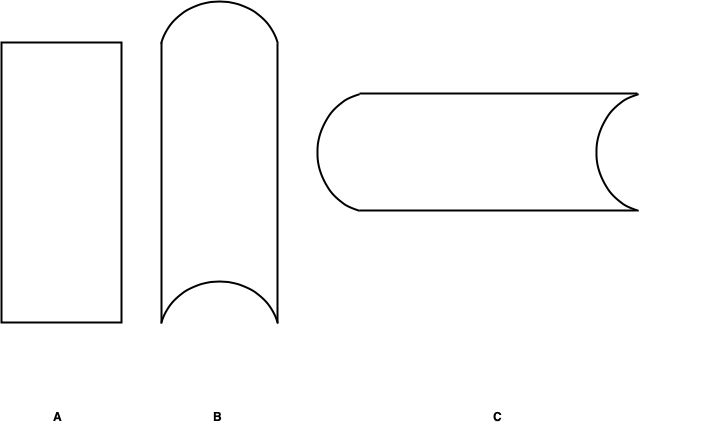
\includegraphics[scale=0.4]{graphics/mirror_type.png}
	\caption{A = planar mirror, B = concave, hemicylindrical mirror with horizontal curvature, C = concave, hemicylindrical mirror with vertical curvature}
	\label{fig:mirror_type}
\end{figure}

Before discussing the three kinds of mirrors, Timaeus provides a general account of the formation of images in mirrors. Mirrors, and other surfaces in which images may be formed, such as the pool in which Narcissus beheld himself, are reflective and smooth (\emph{emphanē kai leia}). Not every surface is receptive to images, only surfaces that meet certain conditions. Being reflective and smooth are conditions on a surface's receptivity to images. Subsequently, Plotinus will be peculiarly sensitive to the general principle implicitly at work hear. An important Plotinian principle (accepted by later Neoplatonists, and promulgated to the Latin West by \emph{Liber de causis}, the Latin translation of the Arabic epitome of Proclus' \emph{Elementa theologica}) is that each receives in accordance with their capacity to receive. Being reflective and smooth is that in virtue of which certain surfaces have the capacity to receive images in the relevant sense. There are three steps to the formation of images in smooth, reflective surfaces. 

% Being reflective and smooth is a necessary condition for the relevant form of image formation. 

First, there is the compounding of the visual body, the combining of inner and outer fire, that extends from the perceiver to the smooth, reflective surface. The compounding of the visual body is a necessary precondition for vision in general, since it is that which receives visual affections, so it is unsurprising that it is involved in the special case of seeing a body reflected in a mirror. When the visual body reaches the smooth, reflective surface, it forms a single fire that can be reshaped (\emph{metarruthmisthentos}) in various ways. \citet[159]{Archer-Hind:1888qd} and \citet[103]{Bury:1929jb} translate \emph{metarruthmisthentos} as deflection, but deformation is clearly meant (see \citealt[287]{Taylor:1928qb}, \citealt[154]{Cornford:1935fk}). Timaeus has in mind the special case of curved mirrors. Curved mirrors present deformed images of what is reflected in them. And since Timaeus is here providing a general account of image formation in mirrors and other reflective surfaces, he must make allowances for these special cases. 

Second, the fire emitted by the colored body, such as a face, extends to the smooth, reflective surface. The fire of the reflected face is its color, since Timaeus conceives of color as a kind of flame (67c–68d). Specifically, color is a power of bodies to emit fire particles that divide (\emph{diakrisis}) or compact (\emph{sugkrisis}) the visual body, or some combination of these. Insofar as a face is colored, it possesses such a power. Timaeus, here, is describing seeing a face in a mirror or some other reflective surface, and not necessarily seeing one's own face \citep[286--7]{Taylor:1928qb}. 

Here questions arise, and I am uncertain how best to answer them. How far, exactly, does the chromatic fire emitted by colored bodies extend? If it extends as far as the surface of a mirror or some other reflective surface, surely it would extend to the eye of a perceiver should they be placed where that surface is. And if that is right, then even should there be no daylight, the chromatic fire could reach the surface of the eye. Why, then, could the chromatic fire not act upon the fire emanating from within directly, there, on the surface of the eye? Begin with the thought that the role of daylight is to connect and so mediate the fire emanating from within the eye with the chromatic fire of the colored body (Proclus, \emph{In Timaeum} 3.1.8 1--7). Timaeus explicitly claims that the fire emanating from within the eye compounds with the daylight. Perhaps the implicit thought, nowhere made explicit in Timaeus' speech, is that daylight's mediation also requires the chromatic fire itself to compound with the daylight. Only in this way, one might think, is the daylight an essential aid and support to vision. If so, then the envisioned possibility would be no possibility at all. However, the body proper to the day and the chromatic fire are different kinds of fire. The former is a mild light that does not burn, whereas the latter is a kind of flame. Is sharing a common genus sufficient for like's affinity for like to effect the compounding, or would the difference in species prevent this? If like cannot act upon like, then since the chromatic fire acts upon the visual body, it would seem that the difference in kind of fire is sufficient for being unlike. In which case there is no compounding of daylight and chromatic fire (since the principle of compounding is like's affinity for like). But then our original question remains, why could the chromatic fire not act upon the fire emanating from within directly, on the surface of the eye?

Third, the fire of the colored body and the fire of the visual body come together (\emph{sumpagous}) on the smooth, reflective surface resulting in the appearance of an image. As we shall see (chapter~\ref{sec:the_eyes}), Timaeus describes the affection of the visual body by the chromatic fire as division  or compaction or some combination of these (67c–68d). So \emph{sumpagous} is not Timaeus' description of the affection that befalls the visual body when seeing. Nor are the two fires compounded in a unified homogenous body, extending between the perceiver and the face whose reflection is seen. On this view, the unified homogenous body receives a motion or affection from the colored body, but it is the chromatic fire that issues from it that affects the visual body, and not the colored body, at least in the first instance.  Rather, the visual body and the chromatic fire meet and come into conflict on the smooth and reflective surface, with the chromatic fire acting upon the visual body, either dividing or compacting it, or some combination of these, thus causing the face to appear to the perceiver in the mirror.

With respect to reflections in planar mirrors, Timaeus' mechanical explanation can be represented as in figure~\ref{fig:mirror}.
\begin{figure}[htbp]
	\centering
		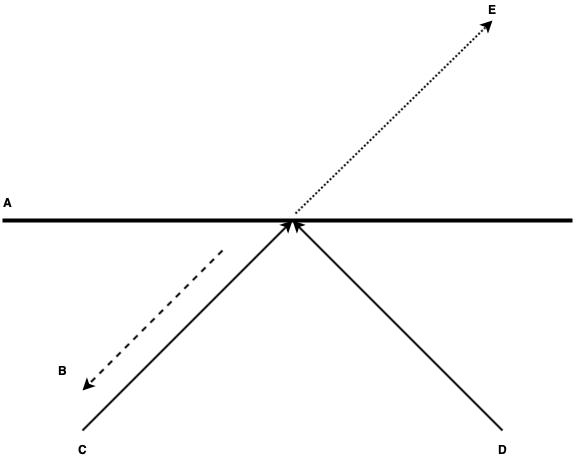
\includegraphics[scale=.4]{graphics/mirror.png}
	\caption{A = surface of the planar mirror, C = the visual body (\emph{opsis}) compounded in the direction that the perceiver is looking, D = chromatic fire emanating from the colored body that appears in the reflection, B = the chromatic \emph{pathēma}, the affection that results from the chromatic fire acting upon the visual body as a whole, E = the image on the surface of the mirror}
	\label{fig:mirror}
\end{figure}
Notice that there is no reflection. Neither the visual body nor the chromatic fire is described as being reflected off the surface. Rather, the visual body and the chromatic fire meet at the surface of the mirror, thus allowing the burning chromatic fire to act upon the mild light of the visual body. Thus \citet[159]{Archer-Hind:1888qd} and \citet[103]{Bury:1929jb} were wrong to translate \emph{metarruthmisthentos} as deflection. There is no reflection or deflection described. The mechanics of Timaean catoptrics is misrepresented in this way in Zeyl's \citeyearpar[34 n 45]{Zeyl:2000cs} diagram as well. It also adds, unprompted, an anachronistic element. The image, E, is represented as projected in the virtual space of the mirror along the line of sight (see figure~\ref{fig:mirror_z}). Nothing in Timaeus's speech suggests as much. Rather, the image in which the colored body appears is on the surface of the mirror where the two fires meet.

\begin{figure}[htbp]
	\centering
		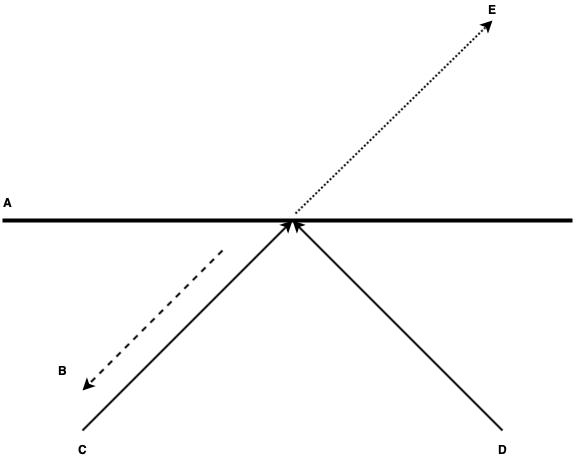
\includegraphics[scale=0.4]{graphics/mirror_z.png}
	\caption{A = surface of the planar mirror, C = the visual body (\emph{opsis}) compounded in the direction that the perceiver is looking, D = chromatic fire emanating from the colored body that appears in the reflection, B = the chromatic \emph{pathēma}, the affection that results from the chromatic fire acting upon the visual body as a whole, E = the image projected in the virtual space of the mirror along the lines of sight}
	\label{fig:mirror_z}
\end{figure}

Timaeus describes three kinds of mirrors and the ways that these orient the reflected image.

Planar mirrors are flat, smooth, reflective surfaces (A in figure~\ref{fig:mirror_type}). In planar mirrors, left appears as right and right appears as left (though up does not appear as down, see \citealt{Block:1974tk}). What explains the reorientation involved in image formation in planar mirrors? Timae\-us' idea is that a part of the visual body meets the opposite part of the chromatic fire issuing from the face. So the right part of the visual body encounters the left part of the chromatic fire, and the left part of the visual body encounters the right part of the chromatic fire, and this gives rise to left appearing right and right appearing left (see figure~\ref{fig:transform}).

\begin{figure}[htbp]
	\centering
		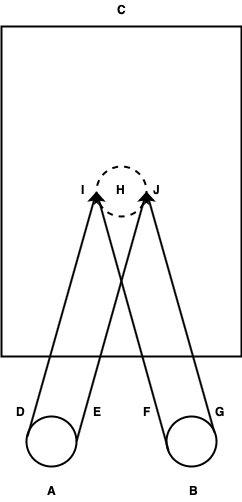
\includegraphics[scale=0.4]{graphics/transform-2.png}
	\caption{A = the perceiver, B = the colored body, C = the planar mirror, D = the left part of the visual body (\emph{opsis}), E = the right part of the visual body, F = the left part of the chromatic fire, G = the right part of the chromatic fire, H = the image on the surface of the mirror, I = the point on the image where the left part of the visual body D meets the right part of the chromatic fire F, J = the point of the image where the right part of the visual body E meets the right part of the chromatic fire G}
	\label{fig:transform}
\end{figure}

Images formed in concave, hemicylindrical mirrors with horizontal curvature, however, are properly oriented with respect to left and right. Such mirrors are concave, so that they bulge inward. They are hemicylindrical and so half a cylinder. And they have a horizontal curvature as when the length of the hemicylinder is vertically aligned (B in figure~\ref{fig:mirror_type}). In such a mirror, right appears as right, and left appears as left. Why do such mirrors differ from planar mirrors? Timaeus says that the chromatic fire switches sides in the process of coming together with the visual body on the curved surface. So the left part of the chromatic fire issuing from the face is reflected to the right, and the right to the left, with the result that the left part of the visual body is affected by the left part of the chromatic fire and the right part of the visual body is affected by the right part of the chromatic fire. And this gives rise to the appearance of an appropriately oriented image (at least with respect to left and right, see figure~\ref{fig:hemicylinder}).

\begin{figure}[htbp]
	\centering
		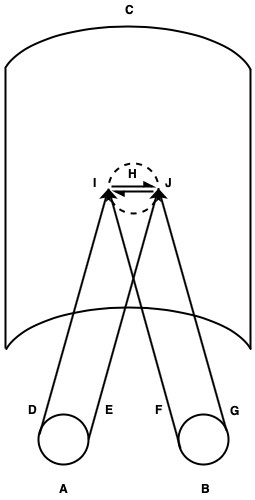
\includegraphics[scale=0.4]{graphics/hemicylinder.png}
	\caption{A = the perceiver, B = the colored body, C = concave, the hemicylindrical mirror with horizontal curvature, D = the left part of the visual body (\emph{opsis}), E = the right part of the visual body, F = left part of the chromatic fire, G = the right part of the chromatic fire, H = the image on the surface of the mirror}
	\label{fig:hemicylinder}
\end{figure}

Should we turn this mirror on its side, however, so that it now comes to have a vertical as opposed to horizontal curvature, up will appear down and down will appear up (C in figure~\ref{fig:mirror_type}). And a parallel explanation is applicable here. The chromatic fire switches sides in the process of coming together with the visual body on the curved surface. Specifically the bottom part of the chromatic fire issuing from the face is reflected to the top, and the top to the bottom, with the result that the top part of the visual body is affected by the bottom part of the chromatic fire, and the bottom part of the visual body is affected by the top part of the chromatic fire. And this gives rise to the face appearing in such a mirror upside down.

Timaean catoptrics is elaborate, if crude. This raises an interpretative question. What is this digression on catoptrics doing here? 

\citet[285]{Taylor:1928qb} observes that Timae\-us uses \emph{phantasmata} to describe both figures in dreams and the images formed in reflective surfaces, suggesting that both are ``unreal''. He also emphasizes the perplexing nature of reflected images. As to the perplexing nature of reflected images, there is reason to think that Timaeus was not particularly puzzled by them. In the first line that introduces the catoptrics, not only does Timaeus explicitly deny that there is any difficulty here, but he does so with pointed irony. ``It is not difficult to see how images are formed in mirrors'' (46a). Timaeus seems to be suggesting that all one need do is look in a mirror and see \citep[47]{Burnyeat:2005rc}. 

\citet[156]{Cornford:1935fk}, like Taylor, connects reflections with dreams and also emphasizes their unreality. He proposes that we understand Timaean catoptrics against the background of a question raised, if unanswered, in the \emph{Sophist} ``How can there be such a thing as a visible world, which is not perfectly real and yet has some sort of existence?'' So understood, the discussion of the catoptrics is well placed in the transition to the discussion of the Receptacle, where the question raised in the \emph{Sophist} will be answered. However, while figures in dreams may be unreal, what we see in mirrors is not. Otherwise why would Demosthenes practice speaking before a mirror (Apuleius, \emph{Pro se de magia} 15)? Indeed, why the evident utility of mirrors in grooming? 

\citet[47--8]{Burnyeat:2005rc} offers a different take. Observing that Timaeus has offered a mechanical explanation of image formation in mirrors and other reflective surfaces ``without a trace of mathematics'', Burnyeat suggests that Plato, in the guise of Timaeus, was engaged in ``a polemic against the idea of a mathematics of visual appearances''. Not even the most elementary facts of a mathematical catoptrics are stated. The Law of Reflection, that the angle of incidence is equal to the angle of reflection, is conspicuous in its absence. Not only does it go unstated, but Timaeus relies on it nowhere is his account. Though the visual body and the chromatic fire are represented as conforming to the Law of Reflection in figure~\ref{fig:mirror}, this principle plays no role in Timaeus' catoptrics, and the Timaean explanation of formation of images in smooth reflective surfaces would remain unchanged even if the Law of Reflection were false. There is further reason, then, to resist \citet[159]{Archer-Hind:1888qd} and \citet[103]{Bury:1929jb} translation of \emph{metarruthmisthentos} as deflection. Not only because it misdescribes the mechanics of Timaean catoptrics, but because of it what it presupposes, that Timaeus is offering mathematical catoptrics.

% section timaen_catoptrics (end)

\section{\emph{Aitia} and \emph{Sunaitia}} % (fold)
\label{sec:_emph_aitia_and_emph_sunaitia}

After the addendum on catoptrics, there is a methodological digression on the distinction between \emph{aitia} and \emph{sunaitia}, causes and auxiliary causes (46c7–
46e6, for discussion see \citealt{Strange:1985aa}). \emph{Aita} has a judicial origin, originally meaning to be held responsible or to be accused. And similarly \emph{sunaitia} originally meant an accomplice, as when Cassandra calls Clytaemestra \emph{sunaitia phonou}, an accomplice to murder, in Aeschylus' \emph{Agamemnon} 1116 as \citet[291]{Taylor:1928qb} observes. In the \emph{Timaeus}, however, these appear, instead, as explanatory notions. (On the judicial origin of Greek explanatory and epistemic notions see \citealt[chapter 4]{Lloyd:1979lc}.) \emph{Aitia}'s significance is perhaps broader than what we would mean more narrowly by cause, but I retain the usual translation as this difference in sense will not prove relevant to our discussion. Despite the opinions of earlier students of nature, what have been discussed so far are not the \emph{aitia} of vision, but merely their \emph{sunaitia} (46d). Most commentators agree that Plato, in the guise of Timaeus, is picking up on an issue raised in the \emph{Phaedo} (96a6--99d2). There, Socrates distinguishes between the \emph{aita} of a thing and a mere necessary condition, that without which the cause would be no cause. Let us begin with the Socrates' account before turning to Timaeus'. Doing so will allow us to highlight an important difference between Timaeus' account and Socrates'. That there be such a difference should not be surprising. Whereas Socrates despairs of cosmology, Timaeus is a keen and ambitious cosmologist.

While sitting in prison, awaiting his execution, Socrates confesses to an early interest in natural philosophy but quickly discovered that he had no aptitude for it. Particularly telling is his encounter with the work of Anaxagoras. According to Anaxagoras, Mind (\emph{nous}) is the cause of all. Socrates confesses that his initial enthusiasm for the Anaxagorean claim was due to a misconception. Socrates had assumed that if Mind is the cause of all, then Mind would arrange everything for the best. But as he became more familiar with Anaxagoras' natural philosophy, Socrates discovered that there was no great difference between Anaxagoras and the Milesian cosmologists. Anaxagoras, like Thales, for example, cites water as a cause. And not only water but air and aether and many other strange things. Anaxagoras seemed to make no use of Mind, and Socrates' early hope that he had found in Anaxagoras a teacher in natural philosophy was dashed. 

The difficulty, according to Socrates, was that the alleged causes cited by Anaxagoras were no causes at all. At best, they were mere necessary conditions without which a cause would be no cause. To dramatize this, Socrates contrasts the cause of his sitting in prison with what are really only necessary conditions for this cause. The cause of Socrates sitting in prison is his decision that it is best that he receives the judgment of his fellow Athenians rather than fleeing. Of course, that his body is composed of sinews and bones is what enables him to sit. Without sinews and bones Socrates could not sit but would merely be piled in a heap (if he could indeed be incarnate in such a pitiful state). But these are not the cause of his sitting in prison. Had Socrates decided instead that it was best to flee, he would have fled with his sinews and bones now enabling him to flee rather than to sit. Thus Socrates draws a distinction between a cause and that without which the cause would be no cause. The majority of natural philosophers and cosmologists fail to mark this distinction. They are thus like people groping in the dark. Moreover, this explains the lack of consensus among them. How could people groping in the dark come to a shared consensus about the explanatory determinants of their common circumstance?

Timaeus, by contrast, seems to realize the ambition for natural philosophy and cosmology that Socrates abandoned. The Demiurge is benevolent and ungrudging and seeks to create the best possible universe. Moreover, he does so exercising \emph{nous}. There are, however, important differences. It would be a mistake to identify the Timaean distinction between \emph{aitia} and \emph{sunaitia} with the Socratic distinction between \emph{aitia} and necessary conditions as \citet[106]{Burnet:1911aa} and \citet[303]{Taylor:1928qb} do. As \citet[104]{Johansen:2004dx} observes, while Socrates thinks that it absurd to describe necessary conditions as causes, Timaeus does indeed so describe them, albeit in a qualified manner. They are \emph{sun\underline{aitia}}. What explains this difference is an important methodological point that Timaeus makes in the present passage. According to Timaeus we should first identify the \emph{aitia} of what we seek to explain and only then go on to identify the \emph{sunaitia}. The \emph{sunaitia} are causes, albeit in a qualified sense, since once we have discovered why things are for the best, we can then go on to identify the necessary conditions for the best to obtain. So understood, these are contributory or auxiliary causes, or ``another kind of \emph{aitia}'' as Timaeus puts it. 

The priority of \emph{aitia} over \emph{sunaitia} is explanatory. The explanatory power of \emph{suniatia} depends upon and derives from the relevant \emph{aitia}. The priority perhaps also applies to the context of discovery. For without a clear conception of the \emph{aitia} a natural philosopher is merely groping in the dark. However, the priority clearly fails with respect to the context of presentation, since Timaeus has, without contradiction or any kind of internal incoherence, presented the \emph{sunaitia} of vision prior to presenting why it is for the best that the young gods have endowed us with eyes to see with.

Indeed, Timaeus inaugurates the methodological digression by observing that so far he has only described the \emph{sunaitia} of vision. Timaeus' predecessors have mistaken these and similar factors, such as heating and cooling, solidifying and melting, as \emph{aitia} of natural phenomena. \emph{Suniaitia} are merely means for perfection. By means of these, an intelligence may bring about the best insofar as it is possible. But \emph{sunaitia}, such as heating and cooling, solidifying and melting, are, by themselves, without intelligence. The only things capable of intelligence, and so capable of acting purposefully to bring about the best insofar as it is possible, are endowed with soul. Soul, however, is invisible, whereas fire, air, water, and earth, are visible. Indeed, we have seen how Timaeus derived the elemental composition of the corporeal from the assumption that the corporeal is visible and tangible. (Strictly speaking, primary bodies, understood as individual polyhedra, are invisible though aggregates of these may be visible. No matter how much Being, Sameness, and Difference the Demiruge mixes, however, the resulting soul stuff will remain invisible.) So explanations invoking only the primary bodies and their powers are incapable, by themselves, of explaining why things are so ordered to produce the best possible result. It is precisely for this reason that the lover of reason and knowledge must prioritize \emph{aitia} over \emph{sunaitia}. Though Timaeus, unlike Socrates, understands necessary conditions as genuine, if qualified causes, he does so in order to realize the Socratic ambition of understanding the cosmos in terms of what is best insofar as that is possible. 

The \emph{aitia} and \emph{sunaitia} may be \emph{explanans} but what, precisely, in the case of vision, is the \emph{explanandum}? What is explained is less particular episodes of seeing than our being endowed with sight by the young gods. Thus Timaeus describes the \emph{sunaitia} of vision as that which helps the eyes acquire the power of sight (46E7). So, for example, the young gods made our eyes light-bearing and of the same kind of mild light that does not burn that composes the body proper to the day in order to endow us with the capacity for sight. Similarly, the \emph{aitia} of vision, the greatest benefit of sight, explains why the young gods endowed us with eyes to see with \citep[107--9]{Johansen:2004dx}. Two observations are relevant here. First, it is sight rather than seeing that is explained. Second, it is the young gods endowing us with sight that is the fundamental \emph{explanandum}.

Though occurring in a section of Timaeus' speech dedicated to the work of Reason (27d--47e), Timaeus' account of the \emph{sunaitia} of vision concerns, not Reason \emph{per se}, but Reasons's exploitation of Necessity for its own purposes. Thus Timaeus claims that all but a small portion of this section has been dedicated to the works of Reason (47e3--4). The small portion being, of course, the discussion of the \emph{sunaitia} of vision. The occurrence of this discussion just prior to the section of Timaeus speech dedicated to the work of Necessity (47e--69a), is twofold. First, the \emph{aitia} of vision, why the young gods endowed human beings with eyes to see with, is, in fact, the work of Reason. As we shall see, sight is providentially provided to produce the best universe insofar as that is possible. Since the \emph{aitia} of vision is legitimately the work of Reason, it properly belongs in the present section. There is, however, a subsidiary motive. In marking the distinction between \emph{aitia} and \emph{sunaitia}, Timaues highlights the post-cosmic form of Necessity, \emph{sunaitia}, not merely a wandering cause, aimless without the purpose of Reason, but Necessity persuaded by Reason to act for the best. In this way is the principle theme of the subsequent section anticipated.

% section _emph_aitia_and_emph_sunaitia (end)

\section{The End of Vision} % (fold)
\label{sec:the_end_of_sight}

Timaeus begins by describing the benefits that vision provides us, describing it as a gift of God. Indeed, vision is described as the cause of the greatest benefit to us without which even Timaeus' present speech would not be possible. Specifically, if human beings had never seen the stars or the Sun or the Heavens, then the kind of cosmology that Timaeus is presently engaging in would not be possible. By means of sight we discern day and night, months and years. Observing the revolutions of the Heavens has four benefits (47a2--b5):
\begin{enumerate}[(1)]
	\item It prompts us to develop the art of number (47a6--8)
	\item It gives us the very concept of time (47a8--9)
	\item With the art of number and the concept of time, we have at our disposal the means to produce accounts of nature (47a8--9)
	\item In deploying our reason in the pursuit of these, we develop a capacity to engage even in philosophy (47a9--b5)
\end{enumerate}
The list of benefits are in ascending order of goodness, culminating with philosophy, which surpasses in value any other divine benefit. Not only is the list in ascending order of goodness, but it also describes a kind of dependency with later items on the list depending on the earlier items.

(1) First, observing the revolutions of the Heavens prompts us to develop the art of number. Consider only the simplest of cases. By means of sight we may observe the passing of day into night and night into day. Moreover, these may be counted. In counting the cycles of day and night we acquire at least a rudimentary conception of number. The revolutions of the Heavens provide measures of not only days, but of months, and years, as well. Not only may these be counted, but arithmetical reasoning may be used to calculate their reoccurrence. 

(2) Second, given that the revolutions of the Heavens are a measure of time, if we possess the art of number, in observing the motions of the Heavens and numbering them, we acquire the concept of time. Here too arithmetical reasoning is fruitfully deployed. Thus our acquisition of the concept of time depends upon our prior acquisition of the art of number.

(3) Third, once we possess the art of number and the concept of time, we possess the means to carry out the kind of detailed investigation into nature characteristic of natural philosophy and cosmology. Thus the study of nature depends upon both the art of number and our concept of time.

(4) Finally, in exercising our reason in acquiring the art of number, the concept of time, and deploying these in the study of nature, we become capable even of philosophy. Thus, according to Timaeus, our capacity to engage in philosophy depends upon our acquisition of the art of number, the concept of time, and our deployment of these in the study of nature. Each of these involve the exercise of reason, and humans, having habituated themselves to the use of reason, become, over time, capable even of philosophy. Philosophy, then, is the greatest benefit of vision. And, in an echo of Euripides, Timaeus claims that a non-philosopher that complains of their loss of sight utters vain lamentations (\emph{Phoenissae} 1762). Apparently, the lesser benefits pale in comparison. (This might seem absurd to moderns if we think of the narrow academic discipline, even to moderns who are practitioners of that discipline, but clearly by \emph{philosopia} Timaeus has in mind a virtuous way of life governed by reason. On philosophy as a way of life see \citealt{Hadot:1997aa,Hadot:2002aa} and \citealt{Cooper:2012aa}.)

Allow me to make some observations. First, Timaeus' does not mention all of vision's benefits. Absent from his list are lesser benefits. Prominent among the unmentioned lesser benefits is vision's utility in navigating a complex environment filled with strong powers that may age, weaken, or even destroy a mortal living being. This is a way in which vision is the forethought of the soul. It is not that Timaeus does not acknowledge the lesser benefits of vision, it is just these pale in comparison with the acquisition of \emph{philosophia}. Second, the benefits that Timaeus mentions are all arts that involve expertise. This is not so of all the lesser unmentioned benefits. Third, philosophy differs from the rest in its degree of independence from the perceptible and the opinable. The other benefits either concern these (the concept of time, the study of nature) or at least have application to them (the art of number). Fourth, though being endowed with sight makes these benefits possible, these benefits involve the exercise of non-sensory powers as well. Specifically, they all involve the exercise of reason.  Fifth, though these are genuine benefits, and philosophy is the greatest, Timaeus does not yet say that the young gods endowed humans with sight so that they may be the recipients of these benefits \citep[107]{Johansen:2004dx}. So Timaeus has not yet said that they are the \emph{aitia} of vision. And if they are not, then we remain in the dark about the true cause and purpose of vison and its benefits.

The \emph{aitia} of vision does not consist in any of these benefits in and of themselves. The \emph{aitia} of vision is not an art requiring expertise and the exercise of reason but is rather a means of psychic regulation (47b5--c4). The young gods endow us with eyes to see with, so that we may behold the revolutions of the intellect of the Heavens, the fixed Stars being moved by the Circle of the Same, and the wanderers, the planets, being moved by the Circle of the Different. The World-Soul and the human soul are alike. Indeed they are akin, the human soul being generated from the same material, if less pure, than the World-Soul, with the Demiurge Father to both. Not only are they generated from the same material but they are similarly constructed. Each is composed of the Circles of the Same and the Different. However, whereas the Circles of the Same and the Different in the World-Soul are unwaverable, their motions constant and invariant, the Circles of the Same and Different in our souls are waverable, and so capable of distortion in the shock of embodiment. The World-Soul, being the elder sibling, is a guide to the human soul. The unwavering revolutions of the Circles of the Same and the Different in the World-Soul are the standard by which the revolutions within the human soul are aligned. In beholding the revolutions of the Heavens, and exercising our powers of reason in accurately calculating their movement, we align the Circles of the Same and the Different in our souls with the unwaverable Circles of the Same and the Different in the World-Soul. In this way, we may stabilize the revolutions within ourselves. This is a remarkable soteriology. By observing the revolution of the Heavens, with attentiveness and intelligence, the disturbance of the shock of embodiment may be overcome, and reason and virtue restored.

There is, however, a striking \emph{aporia} that threatens Timaeus' ocular soteriology. The young gods, acting on the Demiurge's behest, providentially provide us with eyes to see with so that the revolutions in our souls may be set aright and so come to be aligned with the revolutions of the World-Soul. But it is hard to see how the \emph{sunaitia} of vision could so much as be necessary conditions for this achievement. Timaeus' thought is, in part, that the Circles of the Same and the Different of the World-Soul are visibly manifest in the revolutions of the Heavens. The fixed Stars are moved by the Circle of the Same, and the wanderers, the planets, are moved by the Circle of the Different. But these are only fully visible at night. And night quenches the fire emanating within by which we see. If the body proper to the day is among the \emph{sunaitia} of vision, then by what means can we see the starry night?

Not only does Timaeus' account fail to explain nocturnal vision of the Heavens, it fails, as well, to explain more mundane cases of sight. Sitting in a darkened room one may see the illuminated scene outside one's window. Suppose this occurs at noon, or in the afternoon with an East facing window. In such cases the daylight will be at the wrong angle to illuminate even a portion of the darkened room. And yet we may see through the darkness and clearly perceive the illuminated scene without. But how could this be? On Timaeus' account, again, the darkness would quench the fire emanating from within and so it would have no chance of compounding with brother daylight to form the visual body (\emph{opsis}). And if the visual body is unformed, it may not be affected, and if it is unaffected, no vision may occur as a result. The difficulty corresponds to one horn of the dilemma that supports Aristotle's claim that it would be better if the coalescence occurred at the surface of the eye rather than at a certain distance (\emph{De sensu} 2 438a28--9). Either daylight extends to the surface of the eye or it does not. In the latter case, the fire emanating from within would meet darkness and would be extinguished, at least by Timaeus' lights (Alexander of Aphrodisias, \emph{In librum De sensu commentarium} 32.23--24, Aquinas, \emph{Sentenciae libri De sensu et sensato} 3). But that is precisely the situation we are in when we view an illuminated scene from a darkened space.

At least with respect to the nocturnal vision of the Heavens, Timaeus has an answer to this difficulty, or thought he did. Notice that the Sun and our eyes share a common \emph{aitia} (\citealt[112]{Johansen:2004dx}). Not only are the Sun and our eyes each light-bearing, and the light born by each is a mild light that does not burn, but they are light-bearing for the same purpose. The gods kindled a light in the second orbit from the Earth.  The light is called ``Sun'', and it makes conspicuous the relative speeds of the eight revolutions. The Sun illuminates the whole Heaven so that living beings endowed with sight might learn the art of number by observing the revolution of the Same (39b2--c1). Just as the young gods endow us with sight so that we may observe the revolutions of the Heavens, the Sun too was created for just this purpose. Notice that the eight revolutions correspond to the seven divisions of the Circle of the Different. So the Sun is said here to only illuminate the wanderers, the planets. So Timaeus, like Parmenides (DK 28B14), claims that the Moon shines with a foreign light. As to the fixed Stars, perhaps, like the Sun, they are self-illuminating. Unfortunately, the contrivance of the young gods is not fit for purpose. When the body proper to the day has withdrawn, and we are engulfed in the Earth's shadow, the Moon and the other wanderers may be illuminated with the light of the Sun, but we are viewing this illuminated scene from a darkened space. And Timaeus' account of vision cannot explain precisely this.

Among modern commentators only \citet[180--1]{Broadie:2012vl} has noticed this difficulty. And while there is no explicit recognition of this difficulty among ancient commentators, perhaps there is an implicit recognition of it. Consider one way in which Aristotle departs from Timaeus. According to Aristotle, the proper object of vision is the visible. And what is visible is either color or what can be described in words but has no name (\emph{De anima} 2.7 418a26). So color is not the sole proper object of vision (though see \citealt[252]{Polansky:2007ly} for a dissenting view). Aristotle's idea is that the visible divides into two classes, that which is visible in the light and that which is visible in the dark. While colors are visible in the light, fungi, horns, and the heads, scales, and eyes of fish are visible in the dark. Philoponous provides an additional example directly relevant to our present difficulty: starlight is visible only in the absence of the Sun's light (\emph{In De anima} 347 11). Call that which is visible in the dark, the luminous. While Aristotle expresses confidence that seeing the luminous is explained by the very same principles that explains seeing the colors (\emph{De anima} 2.7 419a23--4), he fails to make the explanation explicit, and I, for one, cannot make it out (see \citealt[69--73]{Kalderon:2015fr} for discussion). The luminous, that which is visible in the dark, will be taken up by the ancient commentators, many of whom are Platonists. My hypothesis is that, here, they are, among other things, taking up unfinished business of the \emph{Timaeus}.

The \emph{aporia} is particularly puzzling since it is so obvious, at least once one has it in focus. Moreover, though we have been warned that an \emph{eikos logos} need not be perfectly self-consistent and exact, the present \emph{aporia} is not a departure from consistency that is to be expected from an \emph{eikos logos}. The \emph{sunaitia} of vision are only causes insofar as they are the means of achieving the end of vision. But the alleged \emph{sunaitia} of vision are inconsistent with achieving this end and so are, by Timaeus' lights then, no causes at all, not even auxiliary causes. Such an account is not even likely, let alone as likely, if not more, than any other alternative. Moreover, this occurs in the very passage that introduces and illustrates the \emph{aitia}--\emph{sunaitia} distinction. It is hard not to harbor the suspicion that Plato was alive to the \emph{aporia}, and yet allowed Timaeus' account to be subject to it nonetheless \citep[180]{Broadie:2012vl}. What might Plato signal thereby? 

Timaeus' account of the \emph{sunaitia} of vision cannot be coherently combined with his account of the \emph{aitia} of vision. According to \citet[614]{Taylor:1928qb}, ``When we find [Timaeus] falling into inconsistency we may suspect that his creator is intentionally making him `give himself away'.'' So, on Taylor's hypothesis, Plato is signalling that Timaeus account' of the \emph{aitia} and \emph{sunaitia} of vision is not his own. But even if Plato rejects the incoherent combination of the two accounts, he may yet endorse one of them. But which account does Plato reject, and which does he retain, if any? Does Plato retain Timaeus' account of the \emph{sunaitia} of vision and reject his account of the \emph{aitia}? Or does he reject Timaeus' account of the  \emph{sunaitia} of vision, and retain his account of the \emph{aitia}?

The problem with the first suggestion is that without a specification of the \emph{aitia} of vision, there is no reason to think that the auxiliary causes posited by Timaeus are genuine \emph{sun\underline{aitia}}. Things are only ever \emph{sunaitia} relative to an \emph{aitia} to which they are subordinate and serve. This is why the student of nature should first identify the \emph{aitia} of some phenomena before identifying the relevant \emph{sunaitia}. Put another way, there is no \emph{aitia}-independent specification of the \emph{sunaitia} of vision. And so there is no retention of Timaeus' account of the \emph{sunaitia} without specifying some non-Timaean \emph{aitia} that they might also reasonably serve.

The problem with the second suggestion is that light's role in the causal process eventuating in visual perception is a genuine advance of Timaeus' account over Empedocles'. Plato knows this to be the case. Moreover, it is an advance retained by successor accounts such as Aristotle's in \emph{De anima} and \emph{De sensu}. Moreover, it is retained not just by Peripatetic successors, but by Platonists in the commentary tradition as well. This was a genuine contribution to our understanding of vision. Its obviousness, by our present lights, should not blind us to this fact. But it is precisely this feature that makes nocturnal vision problematic, and the \emph{aitia} of vision, posited by Timaeus, unrealizable. 

A third suggestion is that Plato recognized the incoherence of Timaeus' combined account of the \emph{aitia} and \emph{sunaitia} of vision but recognized the attractions of each, leaving the \emph{aporia} for his readers to grapple with, presumably for their edification. Perhaps Timaeus' account of the \emph{aitia} and \emph{sunaitia} of vision is not so much an \emph{eikos logos} as it is an \emph{eikos muthos}. Plato has Timaeus tell a story where the young gods endow humans with eyes to see with so that they may behold the revolutions in the Heavens and so align the Circles of the Same and the Different within. The story is aporetic. And the reader in grappling with the \emph{aporia} exercises their reason, thereby aligning the Circles of the Same and the Different within, at least by Timaeus' lights. Perhaps the \emph{eikos muthos} has, in this way, a performative aspect. Could an aporetic \emph{muthos} of salvation itself be a means of salvation? Even allowing the evident playfulness evinced in parts of the text, it is unclear, at least to me, how seriously we should take this idea.


% section the_end_of_sight (end)

\section{The End of Audition} % (fold)
\label{sec:the_end_of_audition}

Timaeus provides us with no single comprehensive discussion of audition. Indeed, audition is discussed in three different portions of his speech:
\begin{enumerate}[(1)]
	\item (47c–47e) describes the end of audition, the restoration of the revolutions of the soul
	\item (67a–c) describes the nature of sound and hearing, and provides an account of pitch, evenness of tone, and volume
	\item (80a) describes the nature of concordance
\end{enumerate}
As in the case of vision, Timaeus account of audition cannot be completely understood by confining one's attention to just these passages. And it is not just the general claims about the nature of perception that emerge from his discussion of the \emph{pathēmata}, both common and peculiar, that are relevant. Of particular relevance, as well, is his discussion of the liver (see \citealt{Barker:2000dy}).

Just as the young gods endow us with vision so that we may align the revolutions in our soul with the revolutions of the intellect of the Heavens, sound (\emph{phonē}) and hearing are given for the same purpose. Of sound (\emph{phonē}), speech (\emph{logos}) makes the greatest contribution toward this end. Exactly how, however, Timaeus declines to say, though it is not implausible to suppose that the rationality of speech has something to do with it (compare Aristotle's echo of the Timaean thought in \emph{De sensu} 1 437a11). However, Timaeus' focus, here, is less on speech but on \emph{mousikē}. Timaeus states that \emph{mousikē} that is adapted to sound and hearing is given for the sake of \emph{harmonia}. Notice that \emph{mousikē}, here, is a broader notion than what we mean by music. Music, as we understand it, is audible, making the qualification that music is adapted to sound and hearing unnecessary. The qualification is intended to mark off audible \emph{mousikē} from the broader notion of \emph{mousikē} which has to do with a rational mathematical order (on the rationality of the mathematical order see \citealt{Burnyeat:1987ix} and \citealt{Barker:1994mq}; for a different take see \citealt[295--6]{Taylor:1928qb}). 

Audible \emph{mousikē} is given for the sake of \emph{harmonia}. \emph{Harmonia}, here, does not mean harmony in the sense of the simultaneous sounding of concordant notes. Instead it designates musical intervals akin to the intervals that the Demiurge marked off on the World-Soul. Audible \emph{mousikē} is given for the sake of \emph{harmonia} since the motions of \emph{harmonia} are akin to the revolutions in the human soul. Timaeus distinguishes two ways that we may attend to audible \emph{mousikē}. Familiarly, we may do so merely for the sake of irrational pleasure. But we may also attend to audible \emph{mousikē} with intelligence. When we do, we experience not pleasure (\emph{hēdonē}) but delight (\emph{euphrosunē}). It is this latter manner of attending to music that is relevant to soteriology. When, due to the shock of embodiment, the revolutions in our soul are disturbed, these become unharmonious (\emph{anharmoston}). In attending to music with intelligence, we enlist the \emph{harmonia} that we hear and delight in as an ally to restore the \emph{harmonia} in the revolutions in our soul.

The harmonious motions of the World-Soul and the body of the cosmos that it animates are not themselves audible, though the latter as determined by the former may be seen. (The motions of the World-Soul are not directly seen. The World-Soul is a soul, and soul is invisible, and so too, we may conclude, are its motions. It may, however, be indirectly seen since it moves the body of the cosmos which is visible.) The harmonious motions of the World-Soul and the body of the cosmos thus belong to the broader class of \emph{mousikē} having to do with rational mathematical order. Timaeus' idea is not that we hear them directly. What we hear is not the music of the spheres, but only the music that we ourselves produce. This music has the same rational mathematical order as the motions of the World-Soul and the body of the cosmos that it animates. This is no accident, nor should we audaciously assume that it is due to our own genius. That the music that we make has \emph{harmonia} is, instead, due to divine inspiration. It is the gift of the Muses, the daughters of Memory. When, inspired by the Muses, we make music with \emph{harmonia}, and listen to it intelligently, then we can align the revolutions in our soul to it, thus reestablishing order within. Our ability to hear cosmic \emph{harmonia} is thus indirect and divinely mediated.

It is not solely the \emph{harmonia} of audible \emph{mousikē} that can positively influence the revolutions of our soul. In attending to music with intelligence, we can enlist, not only \emph{harmonia}, but the rhythm that we hear as an ally in realigning the revolutions in our soul. That the music that we make can have a rhythm that may positively influence the revolutions in our soul is likewise due to divine inspiration. Rhythm, like harmony, is a gift of the Muses. Given the greater emphasis that Timaeus gives to \emph{harmonia}, we may assume that rhythm is the lesser of the two gifts. But it is a divine gift nonetheless.

Listening with intelligence in a way that yields not pleasure but delight is crucial to audition's contribution to soteriology. How are we to understand it? What is needed here is an account of what is listening with intelligence such that it explains how doing so may correct the revolutions of the Same and the Different in the soul of mortal human beings. Nothing more may be gleaned from the present passage. Listening with intelligence may only be understood once we have understood Timaeus' account of sound and hearing (67a–c, chapter~\ref{sec:the_ears}), his account of the liver (71a3–72c1), as well as the nature of the \emph{phronimon} (chapter~\ref{sec:pleasure_and_pain}).

% section the_end_of_audition (end)

\section{Concluding Observations} % (fold)
\label{sec:concluding_observations_v_a}

Timaeus' account of vision (45b–46c), along with Empedocles' lantern analogy (Aristotle, \emph{De sensu} 2 437b27–438a3 = DK 31B84), are often cited as important sources for the extramission theory. There are earlier antecedents in this tradition as well, notably Alcmaeon of Croton's account of vision. The accounts of Alcmaeon, Empedocles, and Timaeus should be distinguished from the accounts of the mathematicians, such as Archytas, Hero, and Euclid. While the mathematicians understood optics as applied geometry, Alcmaeon, Empedocles, and Timaeus do not. Their focus is not on the geometry of lines of sight and the ways these structure visual appearance, but, rather, on the physiology and psychology of vision. Other than making the minimal assumptions about these to generate the relevant geometry, the mathematicians seem relatively uninterested in the physiology and psychology of vision. Indeed, if \citet{Burnyeat:2005rc} is right, then Timaeus' catoptrics is a polemic that takes as its object the mathematical orientation of Archytas' optics. There are other differences as well. According to Alcmaeon, Empedocles, and Timaeus, there is a fire that emanates from within the eye. The mathematicians, however, understand the visual ray originating from the surface of the eye and not from within (see the way that Apuleius contrasts Timaeus' view with Archytas', \emph{Pro se de magia} 15). And Timaeus' account contrasts with the mathematicians in conceiving of the visual body as a compound of the fire emanating within and the body proper to the day. The mathematicians, by contrast, do not conceive of the visual ray as a compound. (On the variety of extramission accounts of vision, see \citealt{Lindberg:1978lq}.)

Empedocles' and Timaeus' accounts of vision differ in a more fundamental way from the accounts provided by the mathematicians. According to Euclid's third definition of his \emph{Optics}, those things upon which the visual ray fall are seen. And according to Nemesius, ``Hipparchus says that rays extend from the eyes and with their own extremities lay hold on external bodies like the touch of hands'' (\emph{De natura hominis} 7; \citealt[104]{Sharples:2008aa}). The picture that emerges from these and other remarks is that vision occurs when the visual ray comes into contact with the object of perception. On Timaeus' account, however, the extramissive elements do not reach the colored body seen. Moreover, extramission does not suffice for vision. There are further phases of the causal process eventuating in perception. Like Empedocles' account, according to Timaeus, the fire emanating from within is merely a necessary precondition for the subsequent reception of the effect of the chromatic fire. On Timaeus' account, extramission, the emanation of fire within, makes possible the subsequent intromission, the reception of chromatic affection. The fire emanating from within and the compounding of the visual body are not only physiologically significant, as conditions on the reception of the bodily affection, but are psychologically significant as well. In looking one orients oneself so that the object of perception comes into view. Looking is an active, pre-perceptual orientation toward the object of sight (for a contemporary defense of this conception of looking see \citealt[chapter 5]{Kalderon:2018oe}). The compounding of the visual body in the direction that the perceiver is looking is the corporeal manifestation of an active pre-noetic orientation toward the object of sight. On Timaeus' account, the compounding of the visual body fullfils its psychological role by fullfiling is physiological role. The extramissionist physiology is only there to help realize the psychological function of the compounding of the visual body. One looks and one sees. Actively orienting oneself toward the object of sight is corporeally manifest in the compounding of the visual body thus becoming appropriately receptive to affection from without. The affection is the measure of the power of the agent that caused it and vision is the cognizance of this power. Given this, it seems misleading to describe Emepedocles' and Timaeus' accounts of vision as extramission theories, at least in an unqualified manner. (Perhaps this should be unsurprising. ``Extramission'' and ``intromission'' do not so much as describe naturally occurring positions in the history of philosophy of perception, then they are categories of historiography that are perhaps in need of clarification in light of the complexity of this history.)

Rather than being an extramission theory or an intromission theory, at least on the most straightforward understanding of these notions, Timaeus' account, like the account that Socrates attributes to Protagoras in the \emph{Theaetetus} 156a--b, is perhaps better deemed as interactionist (on ancient interactionism see  \citealt{Remes:2014en} and \citealt{Squire:2016aa}). Vision occurs, not solely through extramission, through the fire emanating from within. Nor does it occur solely from intromission, through the reception of the chromatic affection. But, rather, vision occurs through the interaction of the the visual body, compounded from the fire emanating from within and the daylight, and the chromatic fire. When the compounded visual body comes into conflict with with the chromatic fire, the visual body as a whole communicates the motion from the chromatic fire to the body where it is passed around until the power of the agent that caused it is reported to the \emph{phronimon} (colors, as we shall see in chapter~\ref{sec:the_eyes}, are powers of bodies to emit chromatic fire). And it is this report that constitutes vision. Vision, then, is the cognizance of the power of the agent that comes into conflict with the visual body. It is only through this interaction of three fires of two kinds that vision may occur.





% section concluding_observations_v_a (end)

% chapter the_end_of_vision_and_audition (end)
